\subsection{Metriche documenti}
\subsubsection{Indice Gulpease}
Metrica usata per descrivere la leggibilità dei documenti, di seguito viene riportato una grafico con i valori rilevanti di tutti i documenti, si possono notare i valori limite di accettazione e ideale.
\begin{figure}[h]
	\centering
	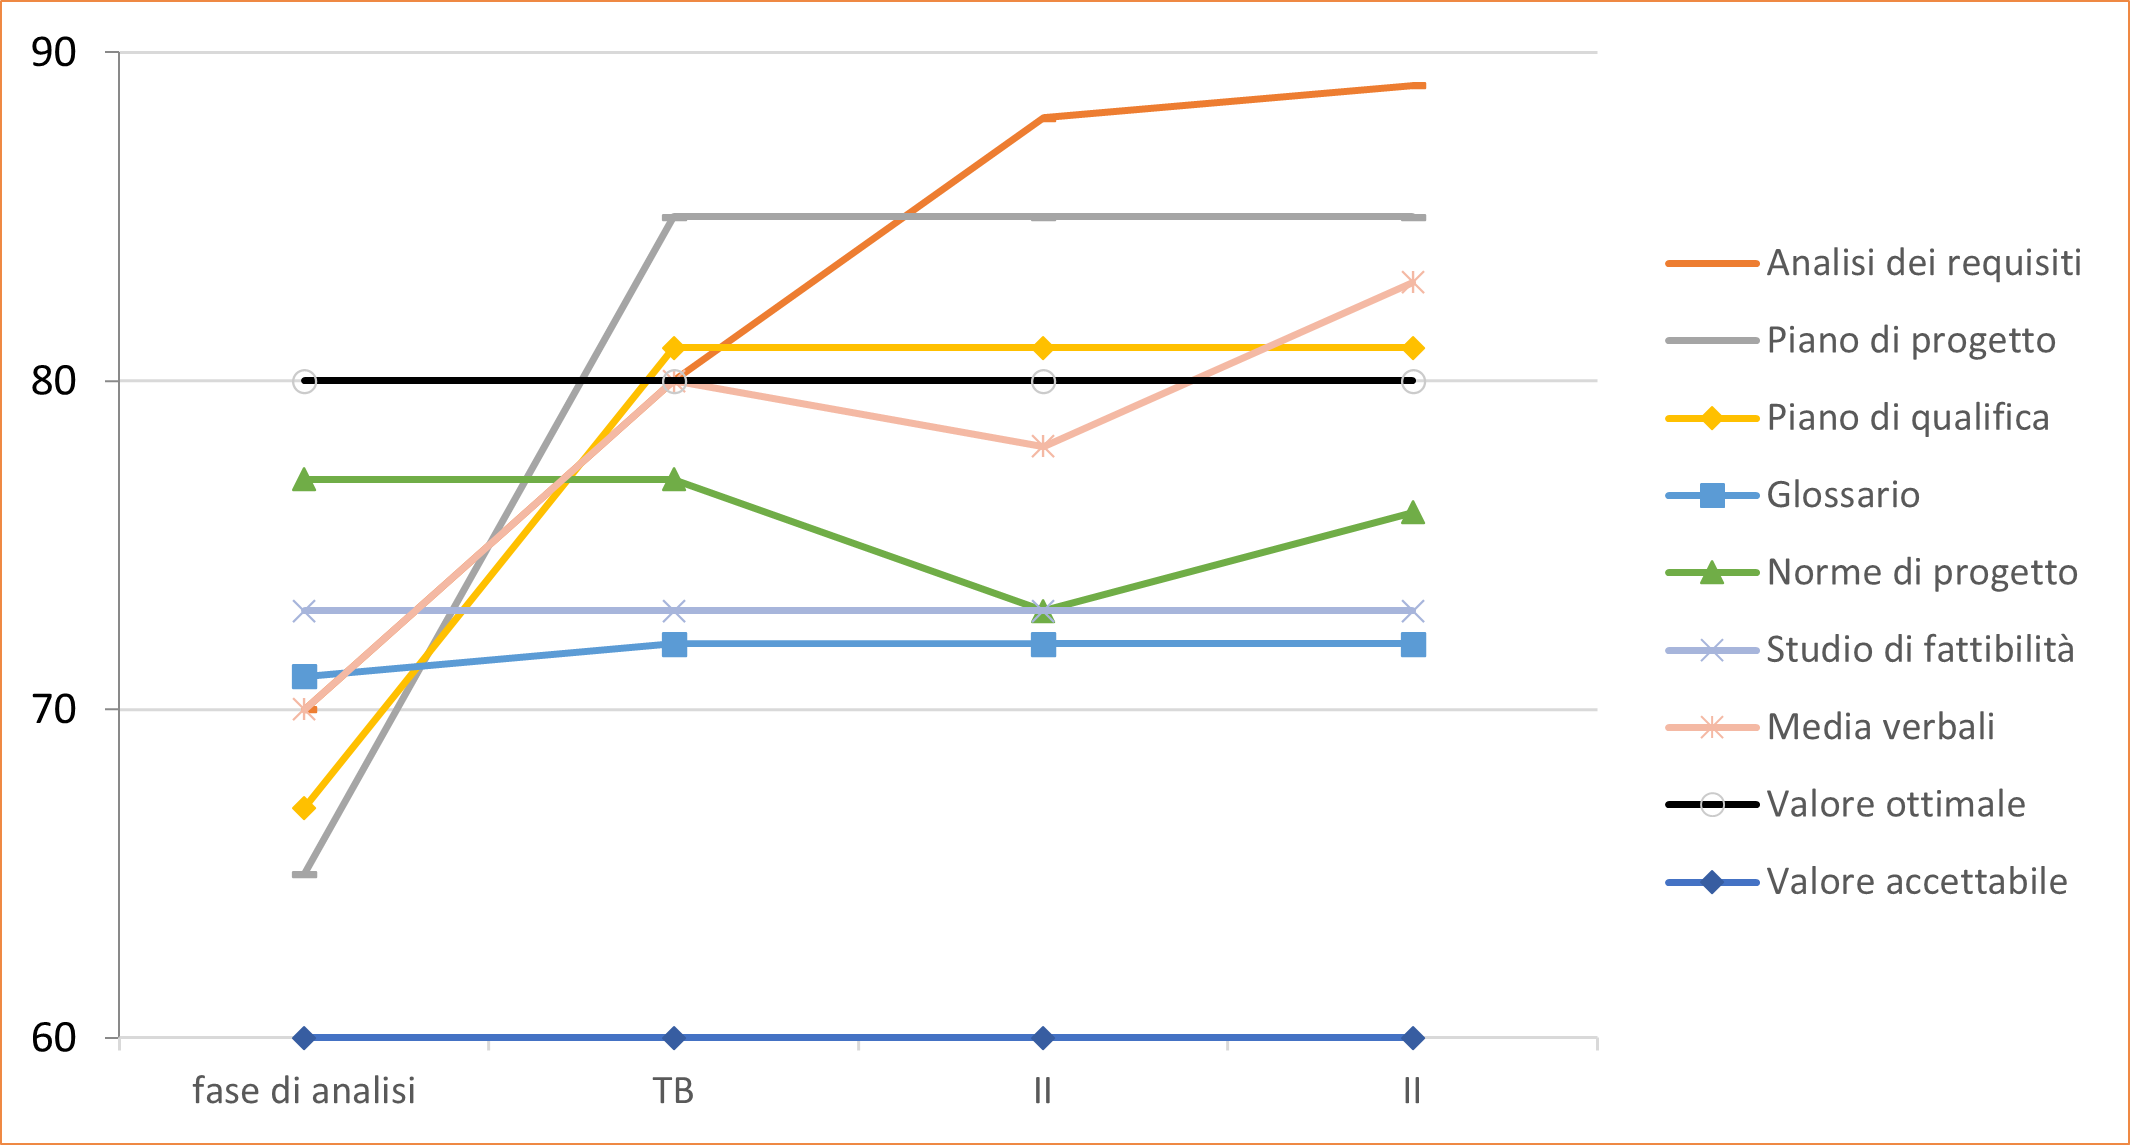
\includegraphics[scale=1]{Images/IndiceDiGulpease.png}
	\caption{Grafico indice di Gulpease nel periodo di progettazione della technology baseline.}
\end{figure}
\subsubsection{Errori ortografici}
Metrica che definisce i risultati della verifica sulla presenza di errori ortografici.
\begin{figure}[h]
	\centering
	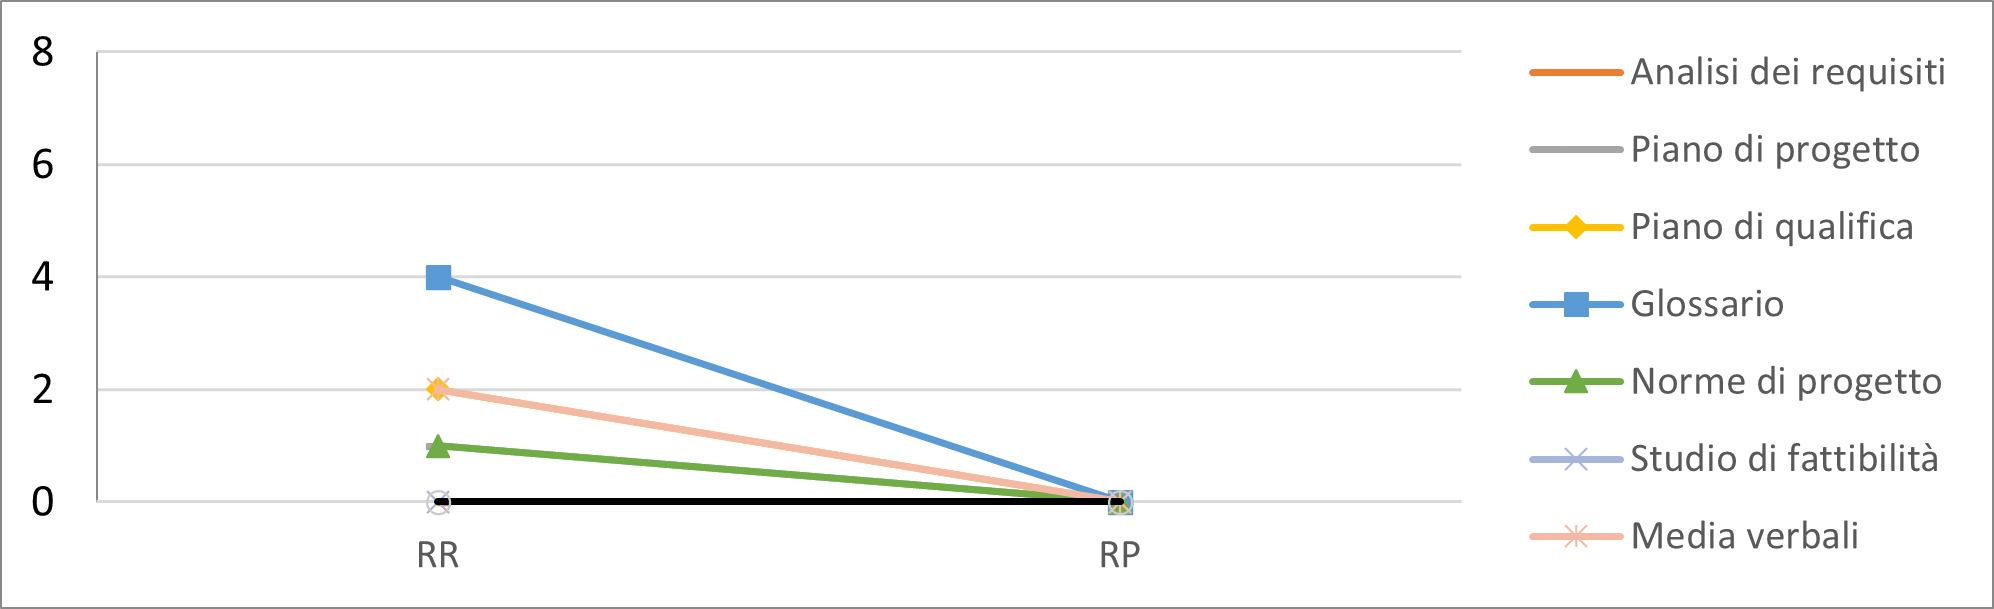
\includegraphics[scale=1]{Images/ErroriOrtografici.png}
	\caption{Grafico degli errori ortografici individuati nelle diverse revisioni.}
\end{figure}